\usepackage[pdftex]{graphicx}
%----------------------------------
\section{System Design}

This section introduces the design of the system modules implemented in sprint 1

%---------------------------------
\subsection{Utility}
The following figure illustrates the current class diagram for this sprint 1.The CSjark module contains the main method of the utility and is responsible for running the program. The utility will typically start off by using cparser to parse the c-header file given to the utility as a command line argument. Cparser will then use the config module to ensure that the parsing is done correctly after the configuration, and then generate protocols and fields to be used in the CSjark module. The CSjark module then generates a wireshark dissector in LUA code by going through the protocols and fields generated earlier by the cparser module. 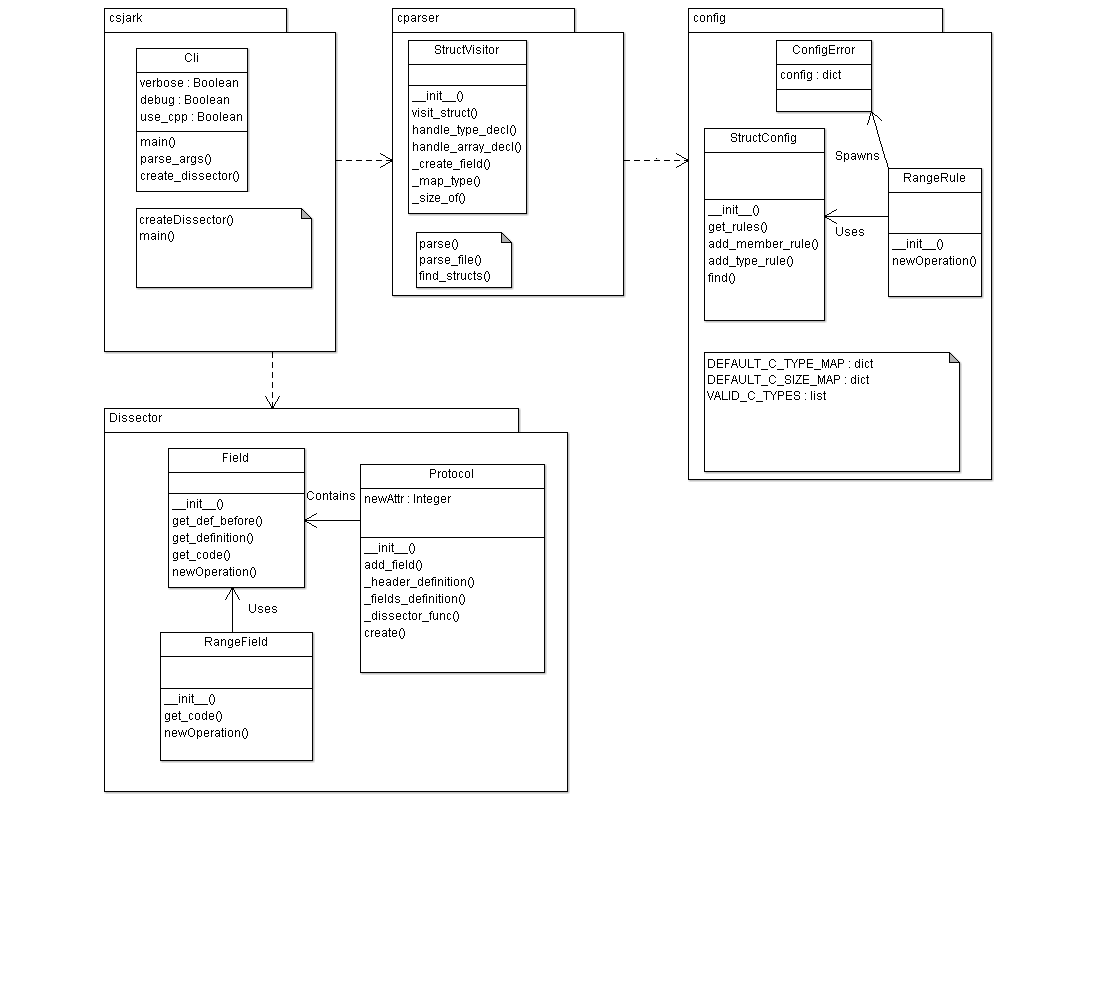
\includegraphics{img\ClassDiagram2.png}





